Hvad kan I lave med 10 blokke?\\
I Figur~\ref{fig:blokke} ser I 10 Scratch blokke.
\begin{figure}
  \centering
  
\includegraphics[height=0.04\paperheight]{glide.png}
  
\includegraphics[height=0.04\paperheight]{go.png}
  
\includegraphics[height=0.04\paperheight]{hide.png}
  
\includegraphics[height=0.04\paperheight]{playSound.png}
  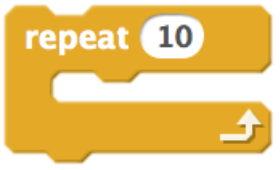
\includegraphics[height=0.08\paperheight]{repeat.png}
  
\includegraphics[height=0.045\paperheight]{say.png}
  
\includegraphics[height=0.04\paperheight]{setSize.png}
  
\includegraphics[height=0.04\paperheight]{show.png}
  
\includegraphics[height=0.04\paperheight]{wait.png}
  
\includegraphics[height=0.055\paperheight]{when.png}
  \caption{10 Scratch-blokke}
  \label{fig:blokke}
\end{figure}
Jeres opgave er at lave et sjovt program kun ved brug af disse blokke. Hver blok må bruges 0, 1 eller flere gange. Prøv at sammensætte programmet ved at tegne blokkene på papir, og skriv ned, hvad I tror programmet vil gøre. Sæt jer dernæst til computeren, og indtast jeres program. Beskriv, i hvor høj grad programmet gør, som I forventede. Vend dernæst tilbage til designfasen og forbedre evt.\ programmet. Til slut uploades programmet til gruppens rum i Scratch.
